\documentclass[a4paper]{article}
\usepackage[utf8]{inputenc}
\usepackage[left=2cm, right=2cm, top=2cm, bottom=3cm]{geometry}
\usepackage{hyperref}
\usepackage[parfill]{parskip}
\usepackage{tikz}
\usetikzlibrary{positioning}

\newcommand{\todo}[1]{\textsf{TODO: #1}}

\title{\textsf{\Huge Draft} \\[3mm] License on Blockchain \\[2mm] \large Transferring and Managing software licenses on the Ethereum blockchain}
\author{Alexander Hoppen, Peter Hoppen}

\begin{document}

\maketitle

\bibliographystyle{abbrvdin}

\section{Overview}

The trade of used software is currently associated with a considerable organisational overhead. Since software licenses are no physical goods, but simply represent the right to use a given software product or are a license key that can easily be copied, on each transaction (transfer) it needs to be made sure that
\begin{enumerate}
  \item the previous owner will not use the license anymore after the transfer has been completed
  \item the previous owner has not sold the license to a different person or organisation
  \item the sold license is genuine and has been issued by the software manufacturer or a certified third party.
  \item Furthermore, the new owner needs to be able to testify that his purchased license is valid by tracing his \emph{used license} to its original issuing.
\end{enumerate}

Currently, all these checks are performed by \emph{used software traders} that are familiar with the kind of software they are trading so that they can verify the validity of the traded licenses. As part of the process they will require the seller to sign that he will not be using the software anymore. Furthermore, they keep a record of all completed transfers so that they can trace any license traded by them back to its original issuing should its genuineness be doubted. 

The above points 1, 2, and 4 are problems that similarly apply to cryptocurrencies like Bitcoin and Ethereum and have been solved for these. In particular 1 and 2 correspond to the problem of \emph{double spending} where the same coin shall not be able to be spent twice and 4 corresponds to the existence of a \emph{digital ledger} that records the entire transaction history.

In this paper we will introduce an approach that allows software licenses to be represented on the \emph{Ethereum blockchain} and which will thus inherit the advances that have been made in the development of this platform. The key problems that will need to be solved are
\begin{itemize}
  \item to find a way to consistently represent software licenses for different software products
  \item to provide a straightforward guideline of how to verify software licenses managed on the blockchain
\end{itemize}

We shall call the framework presented in the following \emph{LOB (License on Blockchain)}.


\subsection{Representation of LOB licenses on Ethereum}

The number of different software products that need licensing is tremendous and it would by no means be possible or feasible to list all of these up-front. Nor should the first licensing of a software product using LOB require any special registration and have a higher overhead than the licensing of existing software products. Hence, we need to create a \emph{framework} that allows the issuing of licenses for \emph{unknown} software products \emph{on demand}. Still, the format of these licenses shall be formalised to standardise the legal and technical aspects to trade these, keeping the organisational overhead as low as possible.

The core of the license's representation will be the \emph{LOB token contract}. It is an Ethereum smart contract template that is compliant to the ERC20 \cite{erc20} standard (ERC 20 describes an interface to trade \emph{tokens} on Ethereum; the concrete meaning of what the token represents is left open by the standard). It will be programmed in a way that makes double spending inherently impossible.

Every time, new software licenses shall be issued using LOB, a new token contract will be instantiated. This token contract will contain a description of the type of software it manages as well as a quantity fixing the number of separately tradable licenses of this type.
 
A license's representation will consist of a human-readable \emph{license name} as well as a \emph{license ID} which may be the software manufacturer's name together with the products stock keeping unit (SKU) or another standardised naming scheme.

These LOB tokens will be tradable as standard Ethereum tokens with standard wallet software. A specialised wallet that automatically verifies the license's validity is still highly recommended though.

Section \ref{ch:tokenContract} will describe the token contract in more detail.

\subsection{Verifying the validity of LOB licenses}

The framework, as described so far, allows everyone to anonymously issue licenses for any software contract in arbitrary numbers without any validation. Furthermore, the issuer may have modified the token contract towards his advantage (e.g. allowing double spending for certain addresses). We will tackle this problem in two steps: Firstly, we will remove the anonymity of token contract creation through \emph{SSL certificates} and secondly, a central \emph{LOB root contract} will issue all token contracts, thus guaranteeing that they have not been tampered with.

\subsubsection{Identifying the LOB license issuer}

By being able to identify the issuer of an LOB license, it is easy to make him liable for the validity of the license in a similar fashion that any reseller is liable for the validity of all licenses he sells. To perform this identification task, we rely on SSL certificates and SSL certificate authorities (CA) that are well established for identification of major websites to prevent phishing.

We require every license issuer to own an SSL certificate that is valid at the time of the license issuing. The issuer will use the private key of this SSL certificate to sign a text (whose content will be described later on and be called the certificate text) and include the signature and his public key in the token contract. Since only he owns the private key and thus only he can have produced the signature, it is guaranteed that he has issued the LOB license.

Should an LOB license not contain a valid signature or the issuer's SSL certificate be invalid (e.g. expired, not issued by a trusted CA), the LOB license is invalid by definition and should not be trusted.

\subsubsection{Preventing corruption of the token contract}

The key building block for a successful transfer of software licenses is the correct functioning of the token contract. The infiltration of a single malicious LOB token contract would greatly harm LOB's reputation. Hence, their correctness must be ensured most thoroughly. The LOB framework shall thus consider no token contract valid unless its code has been written or sanctioned by the LOB mother organisation (whose structure is still to be discussed).

Whether or not a token contract matches source code sanctioned by LOB can be checked in two different ways:
\begin{enumerate}
  \item The wallet software compares the contract's bytecode against a list of valid contract codes and accepts if the bytecode is in that list
  \item A sanctioned \emph{root contract} issues token contracts which always have the same code and only token contracts issued by one of these root contracts are valid
\end{enumerate}

We have decided to use alternative 2 for the following reasons:
\begin{itemize}
  \item Should a vulnerability in a token contract be found, we can create a new root contract and disable the old one, thus preventing the creation of new token contracts with that vulnerability
  \item All token contracts are created from a small list of root contracts and can thus be listed by looking at all outgoing transactions of these root contracts – this will enable wallets to automatically find all token contracts
\end{itemize}

The creation of a new token contract thus works like the following (see figure \ref{fig:tokenContractCreation}):
\begin{enumerate}
  \item The issuer sends a message \texttt{create} to the LOB root contract and passes all parameters necessary, including the license's name and identifier, the quantity, the initial owner, the signature created using his SSL certificate, and the SSL certificate itself
  \item The root contract has the token contract's code hardcoded and creates a new instance
  \item After successful creation of the token contract, it returns the token contract's address
\end{enumerate}

\begin{figure}
  \centering
  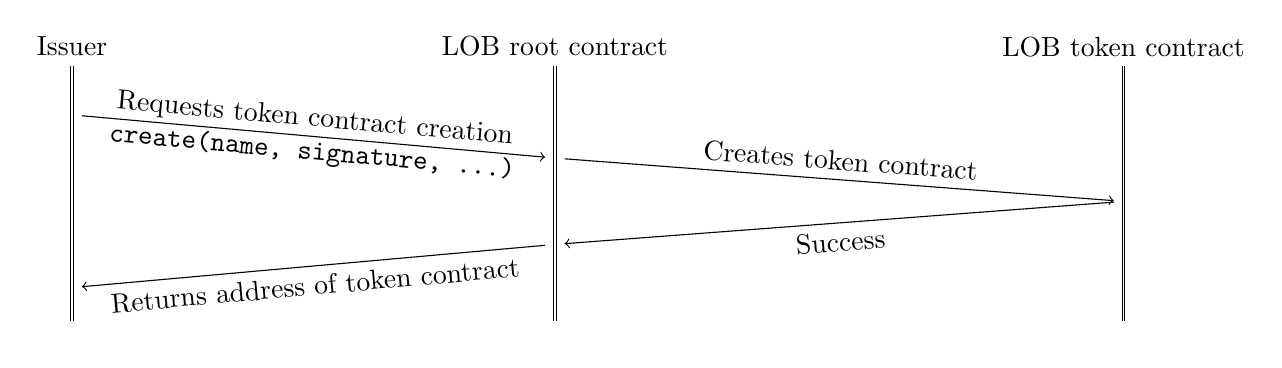
\begin{tikzpicture}[node distance=3mm]
    \node (issuer) {Issuer};
    \node[right=4cm of issuer] (root) {LOB root contract};
    \node[right=4cm of root] (token) {LOB token contract};
    
    \node[below=5mm of issuer] (issuer1) {};
    \node[below=5mm of root] (root1) {};
    \node[below=5mm of token] (token1) {};
    
    \node[below=of issuer1] (issuer2) {};
    \node[below=of root1] (root2) {};
    \node[below=of token1] (token2) {};
    
    \node[below=of issuer2] (issuer3) {};
    \node[below=of root2] (root3) {};
    \node[below=of token2] (token3) {};
    
    \node[below=of issuer3] (issuer4) {};
    \node[below=of root3] (root4) {};
    \node[below=of token3] (token4) {};
    
    \node[below=of issuer4] (issuer5) {};
    \node[below=of root4] (root5) {};
    \node[below=of token4] (token5) {};
    
    \node[below=of issuer5] (issuer6) {};
    \node[below=of root5] (root6) {};
    \node[below=of token5] (token6) {};
    
    \draw[draw, ->] (issuer1) -- node[align=center, sloped] {Requests token contract creation \\ \texttt{create(name, signature, …)}} (root2);
    \draw[draw, ->] (root2) -- node[above, align=center, sloped] {Creates token contract} (token3);
    \draw[draw, ->] (token3) -- node[below, align=center, sloped] {Success} (root4);
    \draw[draw, ->] (root4) -- node[below, align=center, sloped] {Returns address of token contract} (issuer5);
                    
    \draw[double] (issuer) -- (issuer6);
    \draw[double] (root) -- (root6);
    \draw[double] (token) -- (token6);
  \end{tikzpicture}
  \caption{Schematic representation of token contract creation}
  \label{fig:tokenContractCreation}
\end{figure}

\subsection{LOB licenses issuance}

LOB licenses may either be issued as the official software license with the original purchase of the software or \emph{retroactively}. In the latter case, the issuer will verify that the licensee currently owns the \emph{hardcopy license} that was previously issued by the software manufacturer. At the same time the issuer lets the licensee sign that he will not sell the hardcopy license outside the LOB framework and that he will require the same of anyone he should sell the license to. Should any licensee wish to exit the LOB framework, he needs to destroy the LOB license first by invoking the corresponding function on the token contract. A confirmation that the issuer has imposed this restriction on the licensee is included in the certificate text the issuer signs upon the creation of the token contract.

Furthermore, a purchaser may wish to know how trustworthy the issuer is and what liability can be given to this given license. The certificate text thus includes a maximum liability amount given by the issuer and potentially an insurance that guarantees this. Should he have made any mistake in the process of issuing the LOB license, he will reimburse the current owner of the license up to that amount.

In case of a legal dispute it may be necessary that the token contract and all licenses issued with it are revoked (e.g. because the licensee deliberately deceived the issuer by faking the original license and giving wrong statements). In this case, the license's issuer may call \texttt{revoke()} on the token contract, disabling it and rendering all licenses managed by it void. Any reimbursements associated with this action would need to be decided by a court.

\subsection{Linking an LOB license to an installation}

Building on top of the newly created infrastructure, new avenues can be taken. Towards the end, we will describe a method in which the LOB license is transferred into a \emph{software installation} itself. The basic idea is that every installation of the software will generate an Ethereum address and will only function as long as a valid LOB licenses is associated with this address. Thus, to activate the software, one needs to transfer the license to that address, withdrawing the license deactivates the installation. Obviously, each license can only be associated to one address. Hence it is impossible to activate multiple installations using the same license or to sell a license while still using it.

\section{Glossary}

To avoid confusion, some terms that are used in this paper, shall be briefly defined:

\begin{itemize}
  \item \textbf{Hardcopy license:} A software license that already exists but is not managed using LOB (yet)
  \item \textbf{LOB license:} A software license that is managed using LOB
  \item \textbf{Software manufacturer:} A person or company developing and selling software
  \item \textbf{Issuer:} Any person or company issuing LOB licenses, either a software manufacturer or a third party verifying hardcopy licenses
  \item \textbf{Licensee:} The rightful owner of a software license (hardcopy or LOB)
  \item \textbf{Associated address} of an LOB license\textbf{:} The ethereum address that owns a given LOB license. The owner of that address's private key is the licensee.
  \item \textbf{LOB certificate} (short certificate)\textbf{:} A text composed by the issuer that explains the genuineness of the LOB license.
  \item \textbf{SSL certificate:} A RSA/elliptic curve/… certificate issued by a trusted certificate authority which includes the SSL certificate owner's name. Trusted certificate authorities correspond to those trusted by major internet browsers.
  \item \textbf{Address:} An ethereum address backed by either a smart contract or an address in a user's wallet.

\end{itemize}

\section{Smart contract components}

In essence, the LOB infrastructure consists of two smart contracts: 
\begin{itemize}
  \item The \emph{token contract} manages the ownership of a software license and is the central component to trade these
  \item The \emph{root contract} creates new token contracts on the request of issuers and thus ensures that all token contracts have the same implementation
\end{itemize}

Both contracts shall be described in detail below.

\subsection{Token contract}
\label{ch:tokenContract}

For each issuing of software licenses on LOB, a new token contract is created which manages the current owner of these licenses. This means that for a common software like \emph{Microsoft Office}, many different token contracts managing the same type of software may exist. The contract is ERC20-compliant and may thus be traded with common Ethereum wallet software as well as a specialised LOB wallet which additionally verifies the validity of the license as described in section \ref{ch:licenseValidation}. A complete list of methods available in the token contract shall be given in the following.

\todo{It may be cheaper to move all token contract methods into the root contract and let the token contract only have fields for storage. These can only be modified by the token contract. We would lose ERC20-compliance if we do this though}

\subsubsection{Description of the license}

The following fields are getters to arguments passed during the contract's creation and may not be modified afterwards.

\begin{itemize}
  
  \item \texttt{function name() constant returns (string name)}
  \begin{itemize}
    \item Returns a human readable description of the type of license managed by this token contract
  \end{itemize}
  
  \item \texttt{function licenseId() constant returns (string id)}
  \begin{itemize}
    \item Returns an identifier that describes the type of license managed by this token contract
    \item This may be the software manufacturer's name and his SKU or another standardised naming scheme
  \end{itemize}

  
  \item \texttt{function issuer() constant returns (address issuer)}
  \begin{itemize}
    \item Returns the address that initiated the creation of this token contract
    \item This is the address that called \texttt{create} on the root contract
  \end{itemize}
    
  \item \texttt{function issuerName() constant returns (string issuerName)}
  \begin{itemize}
    \item Returns a human readable name of the licenses' issuer
    \item Should match the name in the certificate, if it does not this is a serious indication that the token contract is not trustworthy. Whether or not the names match is not verified on the blockchain because it would require too much computation power.
  \end{itemize}

  \item \texttt{function certificate() constant returns (string certificate)}
  \begin{itemize}
    \item The root contract contains a template for the certificate text with placeholders. The value for these placeholders is stored in the token contract and his function substitutes them in and returns the resulting text
    \item This is the text the issuer has signed with the certificate returned by \texttt{issuerCertificate()}. This signature is returned by \texttt{certificateSignature()}
  \end{itemize}
  
  \item \texttt{function issuerCertificate() constant returns (bytes issuerCertificate)}
  \begin{itemize}
    \item Returns the issuer's SSL certificate and its chain of trust which is used to sign the text returned by \texttt{certificate()}
    \item The following properties are not validated on the blockchain because this would require too much computational power. A breach of any one of these is a strong indication that the token contract is not trustworthy
    \begin{itemize}
      \item Does the data represent a valid SSL certificate?
      \item Is the SSL certificate issued to the issuer? I.e. does the name in the certificate match the name returned by \texttt{issuerName()}?
      \item Has this certificate been issued by a trustworthy certificate authority
    \end{itemize}
    \item \todo{Specify the format the certificate should be in}
    \item \todo{The issuer certificate may be saved in a central database instead of the token contract. This way we would not need to store it over and over again, making the creation of token contracts cheeper.}
    \item \todo{Class 2 certificates are fairly expensive. We should thus also allow class 1 certificates that are less secure and only include an internet domain or email address. In this case the issuerName would not exactly match the name in the certificate (which is the domain or email address)}
  \end{itemize}
  
  \item \texttt{function certificateSignature() constant returns (bytes certificateSignature)}
  \begin{itemize}
    \item Returns the signature created by signing the result of \texttt{certificate()} using the SSL certificate returned by \texttt{issuerCertificate()}
    \item It is not validated on the blockchain whether or not this signature is actually a valid signature of \texttt{certificate()}. If it is not, it is a strong indication that the token contract is not trustworty.
    \item \todo{Specify the format the signature should be in}
  \end{itemize}
\end{itemize}

\subsubsection{License transfer (ERC20 interface):}

\begin{itemize}
  \item \texttt{function totalSupply() constant returns (uint256 totalSupply)}
  \begin{itemize}
    \item Returns the number of individually tradable licenses managed by this token
    \item Decreases as licenses get destroyed using the \texttt{destroy} function
  \end{itemize}
    
  \item \texttt{function balanceOf(address \_owner) constant returns (uint256 balance)}
  \begin{itemize}
    \item Returns the number of licenses currently owned by \texttt{\_owner}
  \end{itemize}
  
  \item \texttt{function transfer(address \_to, uint \_value) returns (bool success)}
  \begin{itemize}
    \item Transfers \texttt{\_value} licenses from the invoker's address to \texttt{\_to}
    \item Triggers the \texttt{Transfer} event with the corresponding parameters
    \item Returns \texttt{true} upon successful transfer of the licenses, \texttt{false} otherwise
    \item Throws if the invoker does not own \texttt{\_value} licenses
    \item Throws if the contract has been revoked
  \end{itemize}
  
  \item \texttt{function destroy(uint256 \_value) returns (bool success)}
  \begin{itemize}
    \item A transfer to nothingness
    \item Subtracts \texttt{\_value} licenses from the invoker's address without granting them to anyone else
    \item Triggers the \texttt{Transfer} event with destination address \texttt{0x0}
    \item Throws if the invoker's address does not own \texttt{\_value} licenses
    \item Throws if the contract has been revoked
  \end{itemize}
\end{itemize}

\vspace{3mm}

The following methods are part of the ERC20 standard and allow the withdrawal of licenses from foreign addresses. They are not part of the LOB workflow yet.

\vspace{3mm}

\begin{itemize}
  \item \texttt{function transferFrom(address \_from, address \_to, uint \_value) returns (bool success)}
  \begin{itemize}
    \item If \texttt{\_from} has allowed the sender to withdraw at least \texttt{\_value} from his account via the \texttt{approve} function, transfers \texttt{\_value} licenses from \texttt{\_from} to \texttt{\_to}.
    \item Triggers the \texttt{Transfer} event with the corresponding parameters
    \item Throws if \texttt{\_from} does not own \texttt{\_value} licenses
    \item Throws if the sender is not allowed to withdraw \texttt{\_value} licenses from \texttt{\_from}
    \item Throws if the contract has been revoked
  \end{itemize}
  
  \item \texttt{function approve(address \_spender, uint \_value) returns (bool success)}
  \begin{itemize}
    \item Approve \texttt{\_spender} to withdraw \texttt{\_value} licenses from the sender's account using the \texttt{transferFrom} function.
    \item Triggers the \texttt{Approval} event with the corresponding parameters
    \item Throws if the contract has been revoked
  \end{itemize}
  
  \item \texttt{function allowance(address \_owner, address \_spender) constant returns (uint256 remaining)}
  \begin{itemize}
    \item Returns the number of licenses \texttt{\_spender} is still allowed to withdraw from \texttt{\_owner}
  \end{itemize}
\end{itemize}

\subsubsection{Revoking the token contract}

\begin{itemize}  
  \item \texttt{function revoke() throws}
  \begin{itemize}
    \item Revoke the licenses certified by this token contract, rendering all license ownerships as void and disallowing any further license transfers. May only be called by the address that created this smart contract (i.e. the root contract in case of the normal LOB workflow)
    
    \item This action cannot be undone. That is `revoked` cannot be set to \texttt{false} again after this function has been called.
    \item Triggers the \texttt{Revoke} event
    \item Throws if called by a different address than the one that created this contract
    \item Throws if the token contract has already been revoked
  \end{itemize}
  
  \item \texttt{function isRevoked() returns (bool revoked)}
  \begin{itemize}
    \item Returns whether or not the token contract has been revoked. If this function returns \texttt{true}, any licenses certified by this contract shall be considered void and not be counted towards the total number of licenses owned by an address
  \end{itemize}
\end{itemize}

\subsubsection{Events}

These events are triggered and thus logged on the blockchain by the corresponding methods. Inspecting the events that have been fired during the token contract's existence allows a detailed reconstruction of the flow of licenses.

\begin{itemize}
  \item \texttt{event Transfer(address indexed \_from, address indexed \_to, uint \_value)}
  \begin{itemize}
    \item Fired for every license transfer
    \item Transfers from \texttt{0x0} represent the creation of licenses, which only happens when the contract is created
    \item Transfers to \texttt{0x0} represent that a license got destroyed
  \end{itemize}
  
  \item \texttt{event Approval(address indexed \_owner, address indexed \_spender, uint \_value)}
  \begin{itemize}
    \item Fired every time a user creates a withdrawal approval via the \texttt{approve} function
  \end{itemize}
  
  \item \texttt{event Revoke()}
  \begin{itemize}
    \item Fired when the token contract gets revoked using the \texttt{revoke} function
  \end{itemize}
\end{itemize}

\subsubsection{Internal data structure}

The token contract keeps a tally that keeps track of the number of licenses associated with any address. All its methods are designed to keep the tally consistent with the number of licenses managed by the token contract and disallow double spending.

\subsection{Root contract}
\label{ch:rootContract}

The root contract's purpose is to generate genuine token contracts that are guaranteed to adhere to the LOB standard and that cannot be manipulated by the issuer towards his advantage. Every Ethereum user can request the creation of a token contract by the root contract and the root contract will adhere to that request. It will not verify the issuer's identity or the integrity of his signature but simply record the parameters it has been given. A verification of the issuer's data is neither wanted nor possible since many decisions (like which CA to trust) are “soft” in that each licensee should be able to make a decision for himself depending on his liability needs. Verification of the certificate's signature also cannot be performed on the blockchain since its computationally too expensive.

The root smart contract contains a template for the LOB certificate whose placeholders will be filled by the issuer and whose entire text will be signed by the user's SSL certificate. Should a new version of this certificate text (e.g. in a different language or because of ambiguities in the original text) become available, a new root contract has to be created and the current one is deactivated if needed. The same holds if a new version of the token contract becomes available.

The usage of a single (or small number of) root contract(s) also has the advantage that all token contracts may be traversed without examining the entire blockchain by simply looking at the root contract's outgoing transactions. This allows wallets to show all licenses owned by an address without the user having to enter the addresses of all token contracts.

For its service, the root contract takes a fee for each contract creation. The amount is still to be fixed. 
A single address is specified as the root contract's owner and is able to withdraw the collected fees and set the fee to a new amount. The owner may also transfer ownership to a new address, e.g. if the LOB root organisation shall be represented by a \emph{distributed autonomous organisation (DAO)} in the future that would be able to vote on how to spend the collected fees.

\textbf{User interface:}

\begin{itemize}
  \item \texttt{function issue(string \_licenseName, uint \_amount, address \_owner, string \_issuerName, string \_remark, string \_liability, bytes \_issuerCertificate, bytes \_certificateSignature) returns (bool success)}
  \begin{itemize}
    \item Creates a new token contract
    \item \texttt{\_licenseName}: A human readable, unambiguous description of the type of software that is licensed; if licenses can only be traded in batches, the batch size; must not be empty
    \item \texttt{\_amount}: The number of separately tradable licenses, must be bigger than 0
    \item \texttt{\_owner}: The initial owner of the licenses
    \item \texttt{\_issuerName}: The name of the human or company issuing the licenses, should match the name in \texttt{\_issuerCertificate} but is not verified on the blockchain. It is the wallet's responsibility to verify its integrity.
    \item \texttt{\_remark}: The text to be filled into the remark placeholder of the license contract
    \item \texttt{\_liability}: The text to be filled into the liability placeholder of the license contract
    \item \texttt{\_issuerCertificate}: The SSL certificate used to sign the license certificate with the given placeholders. Integrity not checked on the blockchain but only in wallet software.
    \item \texttt{\_certificateSignature}: The signature of signing the license certificate (whose exact text may be obtained using \texttt{certificate(…)}). Whether or not the signature actually signs the given certificate text is not verified on the blockchain but only in wallet software.
    \item Returns whether or not the token contract was created
    \item Returns also \texttt{false} if the root contract has been disabled
  \end{itemize}
  
  \item \texttt{function certificate(string \_licenseName, uint \_amount, string \_issuerName, string \_remark, string \_liability) constant returns (string certificateText)}
  \begin{itemize}
    \item Returns the text of the license certificate after substituting in the placeholders
    \item To be used as the basis of the signature in \texttt{\_certificateSignature}
  \end{itemize}
  
  \item \texttt{function fee() constant returns (uint amount)}
  \begin{itemize}
    \item Return the current fee that must be paid to the root contract for each token contract creation; in Wei
  \end{itemize}
\end{itemize}

\textbf{Management interface:}

All of these functions throw unless called by the root contract's owner, unless otherwise specified.

\begin{itemize}
  \item \texttt{function owner() constant returns (address owner)}
  \begin{itemize}
    \item Returns the current owner of the root contract
    \item May be called by anyone
  \end{itemize}

  \item \texttt{function transferOwnership(address \_to)}
  \begin{itemize}
    \item Transfer ownership of this smart contract to \texttt{\_to}
  \end{itemize}

  \item \texttt{function setFee(uint \_amount) throws}
  \begin{itemize}
    \item Set the fee required to create token contracts; in Wei
  \end{itemize}
  
  \item \texttt{function withdraw(uint \_amount, address \_recipient) throws}
  \begin{itemize}
    \item Send \texttt{amount} Wei to \texttt{recipient}
  \end{itemize}
  
  \item \texttt{function disable() throws}
  \begin{itemize}
    \item Disable the root contract so that no more token contracts may be created with it
  \end{itemize}
  
  \item \texttt{function revoke(address \_tokenContract) throws}
  \begin{itemize}
    \item Revoke the software licenses managed by the token contract with the given address by calling \texttt{revoke} on it
    \item May also be called by the issuer of the given token contract
    \item \todo{Should the root contract's owner have the right to revoke a token contract?}
  \end{itemize}
\end{itemize}

\textbf{Events:}

\begin{itemize}
  \item \texttt{event OwnershipTransfer(address \_from, address \_to)}
  \begin{itemize}
    \item Fired when ownership of the root contract changes using the \texttt{transferOwnership(…)} function
  \end{itemize}
  
  \item \texttt{event FeeChange(uint \_newFee)}
  \begin{itemize}
    \item Fired when the fee for token contract creation is changed using \texttt{setFee(…)}
  \end{itemize}
  
  \item \texttt{event Disabled()}
  \begin{itemize}
    \item Fired when the root contract gets disabled using the \texttt{disable()} function
  \end{itemize}
  
  \item \todo{Should token contract creation fire an event? If yes, which parameters should it take, maybe simply recording the token contract's address may be enough}
\end{itemize}

\section{Issuing of software licenses}
\label{ch:licenseIssuing}

The following shall describe the process of issuing an LOB license in more detail. 

\subsection{Phase 1: Validating that owner actually owns license}

In a first step, the issuer of the license needs to ensure that the licensee actually owns the software license whose management shall from now on be performed using LOB. For this, multiple scenarios are possible, including the following.
\begin{itemize}
  \item The LOB license is issued upon purchase of the actual license. The seller of the software license knows by definition that the purchaser owns the license on purchase and can simply issue the LOB license instead of a hardcopy license as part of fulfilling the purchase contract.

  \item Used software traders already have well-established procedures to verify that the instance selling used software to them is not using it anymore. When the used software trader resells the software, it can issue an LOB license as if it were a software manufacturer.

  \item Similarly, any trustworthy third party may perform the validations used software traders perform at the moment, but without purchasing the licenses that shall from now on be managed using LOB. Instead, the third party simply issues the LOB license to the current hardcopy license owner. One crucial aspect of validation the issuer has to perform is that it must certify that the license is not managed using LOB (or any similar system) yet, as to prevent the issuing of multiple LOB licenses for the same hardcopy license. Furthermore, the issuer needs to ensure that the licensee does not sell the hardcopy license without invalidating the LOB license first. This is done by including a paragraph in the root contract's certificate that obliges every LOB purchaser to not sell the license outside the LOB framework without destroying its LOB counterpart first.
\end{itemize}

\subsection{Phase 2: Blockchain transactions}

After the issuer has verified that he wants to issue an LOB license as described in the previous section, it performs the following steps:

\begin{enumerate}
  \item It determines a unique identifier for the license to be managed using LOB. This may be the SKU of the software manufacturer, another standardised naming scheme
  \item It composes a human-readable name describing the type of license
  \item It determines the liability it can give for the LOB license to be backed by a duly purchased hardcopy license (this step is not applicable if the software manufacturer issues the LOB license)
  \item It generates the license certificate text by invoking \texttt{certificate(…)} on the root smart contract
  \item The just returned text gets signed using an SSL certificate issued by a certificate authority. If such a certificate does not exist yet or has expired, the issuer needs to request one before being able to proceed.
  \item The issuer invokes \texttt{issue(…)} with the same parameters that were used on the call to \texttt{certificate(…)}, his SSL certificate, the just generated signature and the Ethereum address of the licensee
  \item After the transaction gets mined, the issuer optionally tells the licensee the address of the newly created token contract together with instructions on how to verify and trade the LOB license (should the licensee already be familiar with LOB, a wallet software may automatically pick up the new token contract by traversing all newly created contracts by the root smart contract)
\end{enumerate}

Optionally, licensee and issuer may set up a smart contract that only generates the LOB license after the licensee has paid the issuer a fee for creating the license to avoid one party not fulfilling its duty.

\section{Validating the ownership of a software license}
\label{ch:licenseValidation}

Verifying all integrity concerns of token contracts on the blockchain is neither advisable due to the high transaction costs to perform expensive computations, nor is it necessary. Some verification steps don't have a single “right” answer but the licensee needs to judge for himself which requirements apply (such as which CA to trust or which liability to require). Wallet software has to guide the user through these validation steps and simplify information as much as possible while still allowing the user to view all information.

The following list shall be a guideline on what checks must be performed to verify that someone owns the LOB license he claims to own. All of the following steps can be performed offline and do not require gas for any transaction to be performed on the blockchain.

\begin{itemize}
  \item Verify that the other party owns the private key of the Ethereum address he claims to possess by giving him a message to sign and verify that the signature can be decrypted using the address's public key
  \item Determine the token contract managing the software license in question either by enumerating all token contracts created by the root contract or asking the licensee for the token contract's address
  \item Call \texttt{balanceOf(…)} with the licensee's address on the token contract and verify that a number of licenses matches (or exceeds) the claimed amount
  \item Check that the token contract has not been revoked
  \item Check that the license name describes the type of license the licensee claims to own
  \item Check that the data returned by \texttt{issuerCertificate()} is a valid SSL certificate
  \item Verify that the name in the issuer's SSL certificate matches the name returned by \texttt{issuerName()}
  \item Is the certificate authority that issued the certificate trustworthy, has the required security level, or has the issuer's SSL certificate been revoked?
  \item Verify that the data returned by \texttt{certificateSignature()} is a valid signature of the text returned by \texttt{certificate()} using the certificate returned by \texttt{issuerCertificate()}
  \item Check that the liability is sufficient
\end{itemize}

\section{Revoking of LOB licenses}
\label{ch:revoking}

In case there is a dispute whether a license is valid or if the licensee has lied to the issuer in the process of issuing the LOB license, it may be necessary that the LOB license is revoked, i.e. invalidated and rendered void. Bearing the right to perform this action carries a great responsibility as it may easily be abused. Since the issuer is already a person of trust for the traded LOB license who would lose his trustworthiness (and thus his business) by arbitrarily revoking LOB licenses, we believe that he is the right candidate to be able to revoke the LOB licenses he has issued. 

Should an LOB license be revoked (e.g. by order of the court), the issuer of that license can invoke \texttt{revoke(…)} on the root contract, which in turn calls \texttt{revoke()} on the token contract, setting a boolean \texttt{isRevoked} flag on the token contract, such that it will be displayed as being revoked in LOB wallet software which also makes it unable to trade these licenses any further. The action cannot be undone. Thus, should a revoke have been performed accidentally, a new token contract needs to be created that has exactly the same certificate parameters as the token contract that has just been revoked.

Should a major security flaw be detected in the token contracts issued by a root contract, the root contract may choose to invalidate all of its token contracts while at the same time a new root contract that contains the bugfix issues new token contracts with exactly the same owners. \todo{Do we really want to do this and have the right to revoke all token contracts?}

Similarly, a license owner may decide that he no longer wants to manage his licenses using LOB, e.g. to go back to hardcopy trading for whichever reason. For this, he needs to destroy his LOB license and can do so by invoking \texttt{destroy(…)} on the token contract.

\section{Use cases}
\label{ch:useCases}

Since licenses are just plain Ethereum tokens, they can be incorporated in further smart contracts, built around LOB. Some potential ideas shall be sketched below. Their full specification is still to be done.

\subsection{Purchase contract}
\label{ch:purchaseContract}

To avoid the trade issue where one party transfers the LOB license to be traded but the other does not pay the agreed amount (or vice versa), the trading parties may agree to set up a smart contract that takes the role of an escrow: Once both parties have transferred the good to be traded to the smart contract, every party can take what used to be the other's property. Should one party not pay, the other party can take his good back. After a successful trade, the smart contract has outlived its use and is no longer needed. No adjustment of LOB is necessary for this.

\subsection{Transfer license to installation}
\label{ch:installationContract}

The LOB licenses as described so far do not prevent the scenario where one license is used to activate multiple installations (when not allowed by license terms). Such a misuse may currently only be discovered when the software manufacturer performs an audit at the licensee. The method described in the following section allows a software installation to verify that the licensee owns a valid LOB license for given software and does not use the same license for multiple installations.

The basic idea is that the LOB license is transferred into the installation in order to activate it. Hence the license is associated with the \emph{installation} and no longer the licensee's address. Since the same license cannot be associated with two addresses, only one installation can be activated with the same license. The license owner still has the right to withdraw the license from an installation at any moment. Should the installation detect that it no longer is associated with the license, it may act accordingly, e.g. by limiting its functionality or refusing to launch.

In detail, the method will be performed like this:

When installing, the software installation creates an Ethereum address and asks the user to transfer a small amount of ether to that address. These Ethers will be needed to set up some helper smart contracts by the installation. Once the Ethers have reached the address, the installation asks for a \emph{management address}, creates an \emph{installation contract} and transfers all remaining ethers to the management address. The installation contract will be the contract to which the LOB license will need to be associated for the installation to be activated. It does not own any Ethers. The installation contract will relay any transaction request sent to it by the management address and may thus be told to transfer the license to another address at any moment. As long as an appropriate LOB license is associated with the installation contract, the installation is activated.

It still needs to be determined which LOB licenses are \emph{appropriate} to activate the installation. A feasible option would be to only accept licenses which contain a fixed SKU as the license's name and are issued by the software manufacturer himself or some trusted third party issuers.

\todo{Can be improved by adding a new method to the token contract that allows transferring the license to a new address while directly approving withdrawal}

% Just sketchy notes, should not be included in the whitepaper
%
%\section{Software rental}
%\label{ch:rental}
%
%
%Rental of software licenses requires the addition of sub-token-contracts. To let $x$ software licenses, they are removed from the normal token contract and a new token contract with exactly the same parameters as the parent contract but with an expiry date is created. A sub-contract's expiry date may never be later than the original contract's expiry date. The original contract saves its sub-contract's address, the original owner and the sub-contract saves the parent contract's address. When a sub-contract has expired, the parent contract can tell the sub-contract to remove all licenses it manages (which it cascades to all its sub-contracts) and adds the licenses back to the original owner.
%
%Maybe the fixed expiry date can be replaced by a custom smart contract to allow more flexible renting schemes.

\section{Validation of license issuers}
\label{ch:licenseIssuerValidation}

To simplify the judgement of whether or not an issuer is trustworthy (checking its liability, SSL certificate, internal standards), an independent institution can verify license issuers, giving them some status of trustworthiness. This list could be managed on a central address on the Ethereum blockchain but is other than by wallet integration not affiliated with LOB.

\bibliography{references}

\end{document}